\clearpage
\newpage
\section{Figures}
\begin{figure}[H]
	\centering
	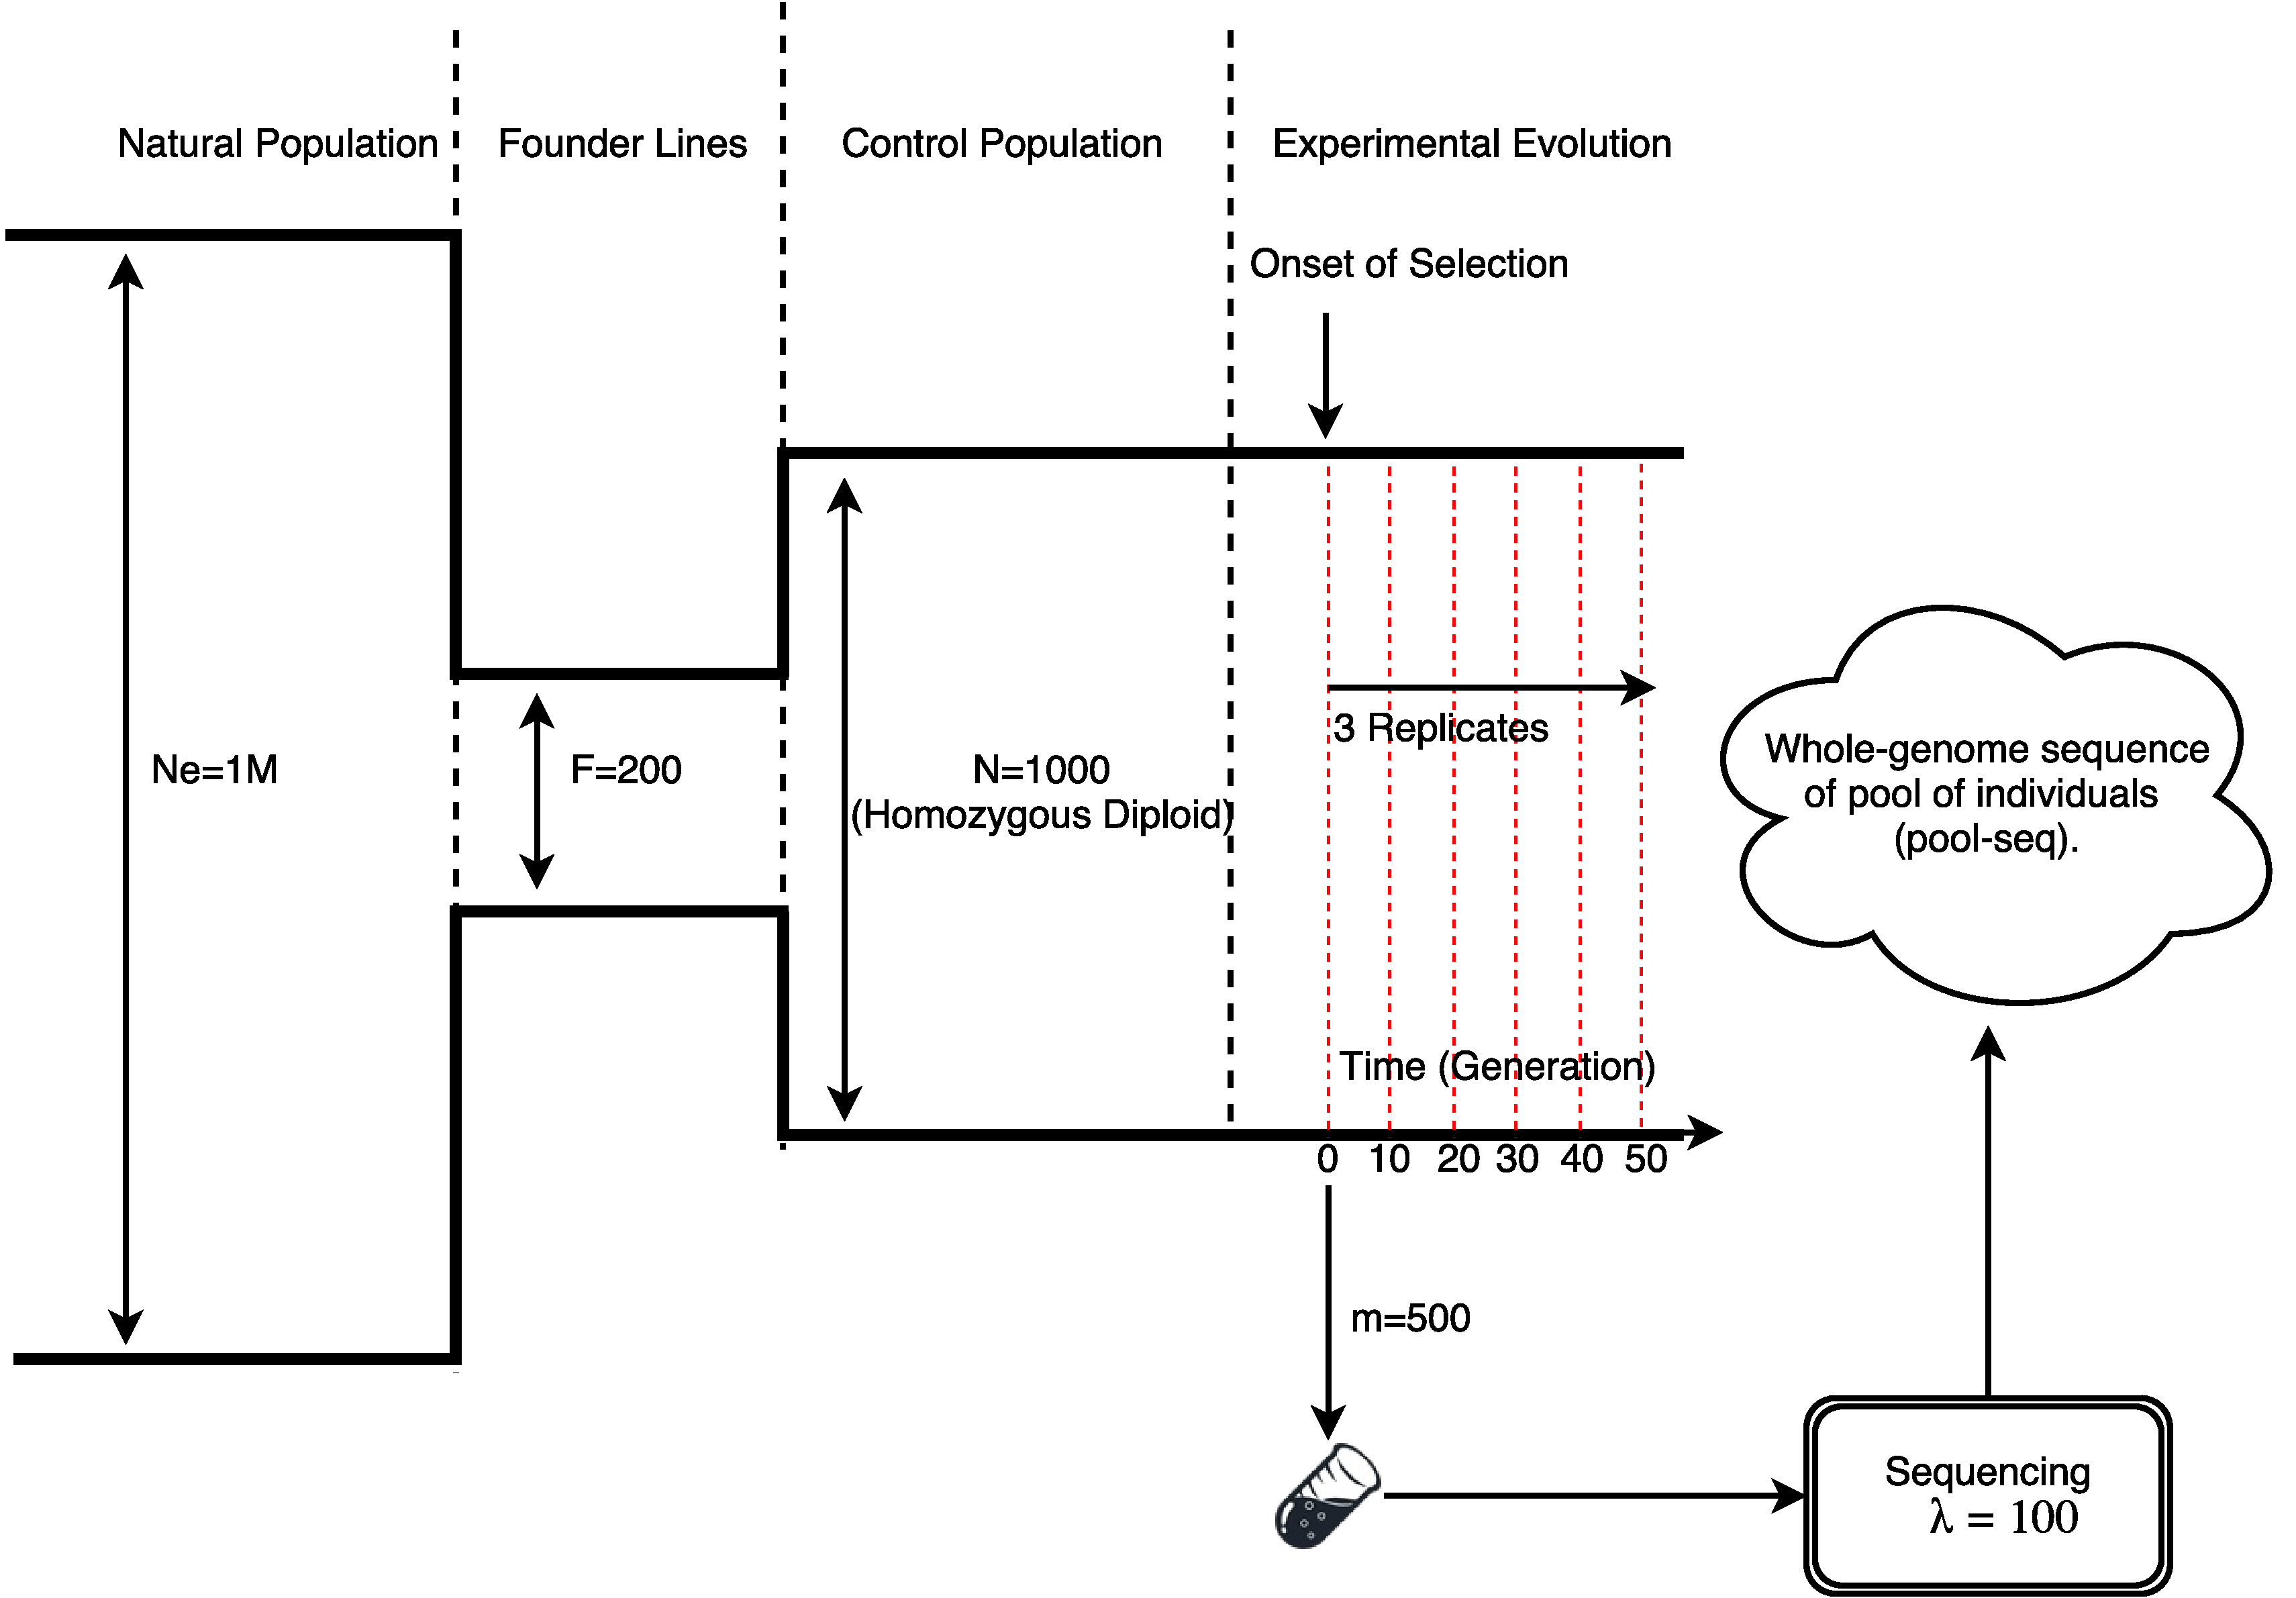
\includegraphics[trim=0.1in 0 .08in 0.02in , 
	clip,width=\textwidth]{ExperimentalEvolution.pdf}
	\caption{ {\bf Two settings for collecting genomic time series            
	data.}\\
		 Different settings in which dynamic data is
          collected are depicted with typical parameters for \emph{D.
            melanogaster}. In both settings, 6 samples (vertical red
          dashed lines) are taken every 10 generation.  When sampling
          from naturally evolving populations (A), the time of onset
          of selection is unknown, and population size is larger. For
          (controlled) experimental evolution (B), founder lines are first
          sampled from a natural population to create a homogeneous
          population. Then, multiple replicates of this population are
          evolved and sampled over time. }
	\label{fig:ee}
\end{figure}


\begin{figure}[H]
	\centering
	\includegraphics[width=\textwidth]{{markovDists}.pdf}
        \caption{{\bf Comparison of empirical distributions of allele
            frequencies (red) versus predictions from Brownian
            Motion (green), and Markov chain (blue).}\\ 
          Comparison of empirical and theoretical distributions under neutral 
          evolution (panels A-F) and 
          selection (panels G-M) with
          different starting frequencies $\nu_0\in\{0.005,0.1\}$ and
          sampling times of $\Tc=\{0,\tau\}$, where $\tau \in \{1,10,100\}$. 
          For each panel, the
          empirical distribution was computed over 100,000 simulations. 
          Brownian motion (Gaussian approximation) provides poor approximations 
          when initial frequency is far from 0.5 (A) or sampling is sparse 
          (B,C,E,F). In addition, Brownian motion can only provide 
          approximations under neutral evolution. In contrast, Markov chain 
          consistently provide a good approximation in all cases.}
	\label{fig:markov}
\end{figure}

\begin{figure}[H]
	\centering
	\includegraphics[trim=.2in 0 .2in 0, 
	clip,width=\textwidth]{{CLRQ}.pdf}
	\caption{{\bf Average power of \comale\ statistics as function
            of percentile cutoffs.}\\ Detection power is averaged for
          $s\in\{0.025,0.05,0.075,0.1\}$ for \comale\ statistics, $\Hc_{\pi}$ and
          $\Hc^{+}_{\pi}$. We denote
          $\pi^{*}=\arg\max_{\pi}\{\mbox{Power}(\Hc),\mbox{Power}(\Hc^{+})\}$. Average
          power was computed using $8000$ simulations for each choice
          of $\pi$. The appropriate choice of $\pi$ can be used to
          improve performance for different coverage values. 
          In all simulations, 3 replicates are evolved and sampled at generations 
          $\Tc=\{0,10,20,30,40,50\}$.}
	\label{fig:clrq}
\end{figure}

\begin{figure}[H]
	\centering
	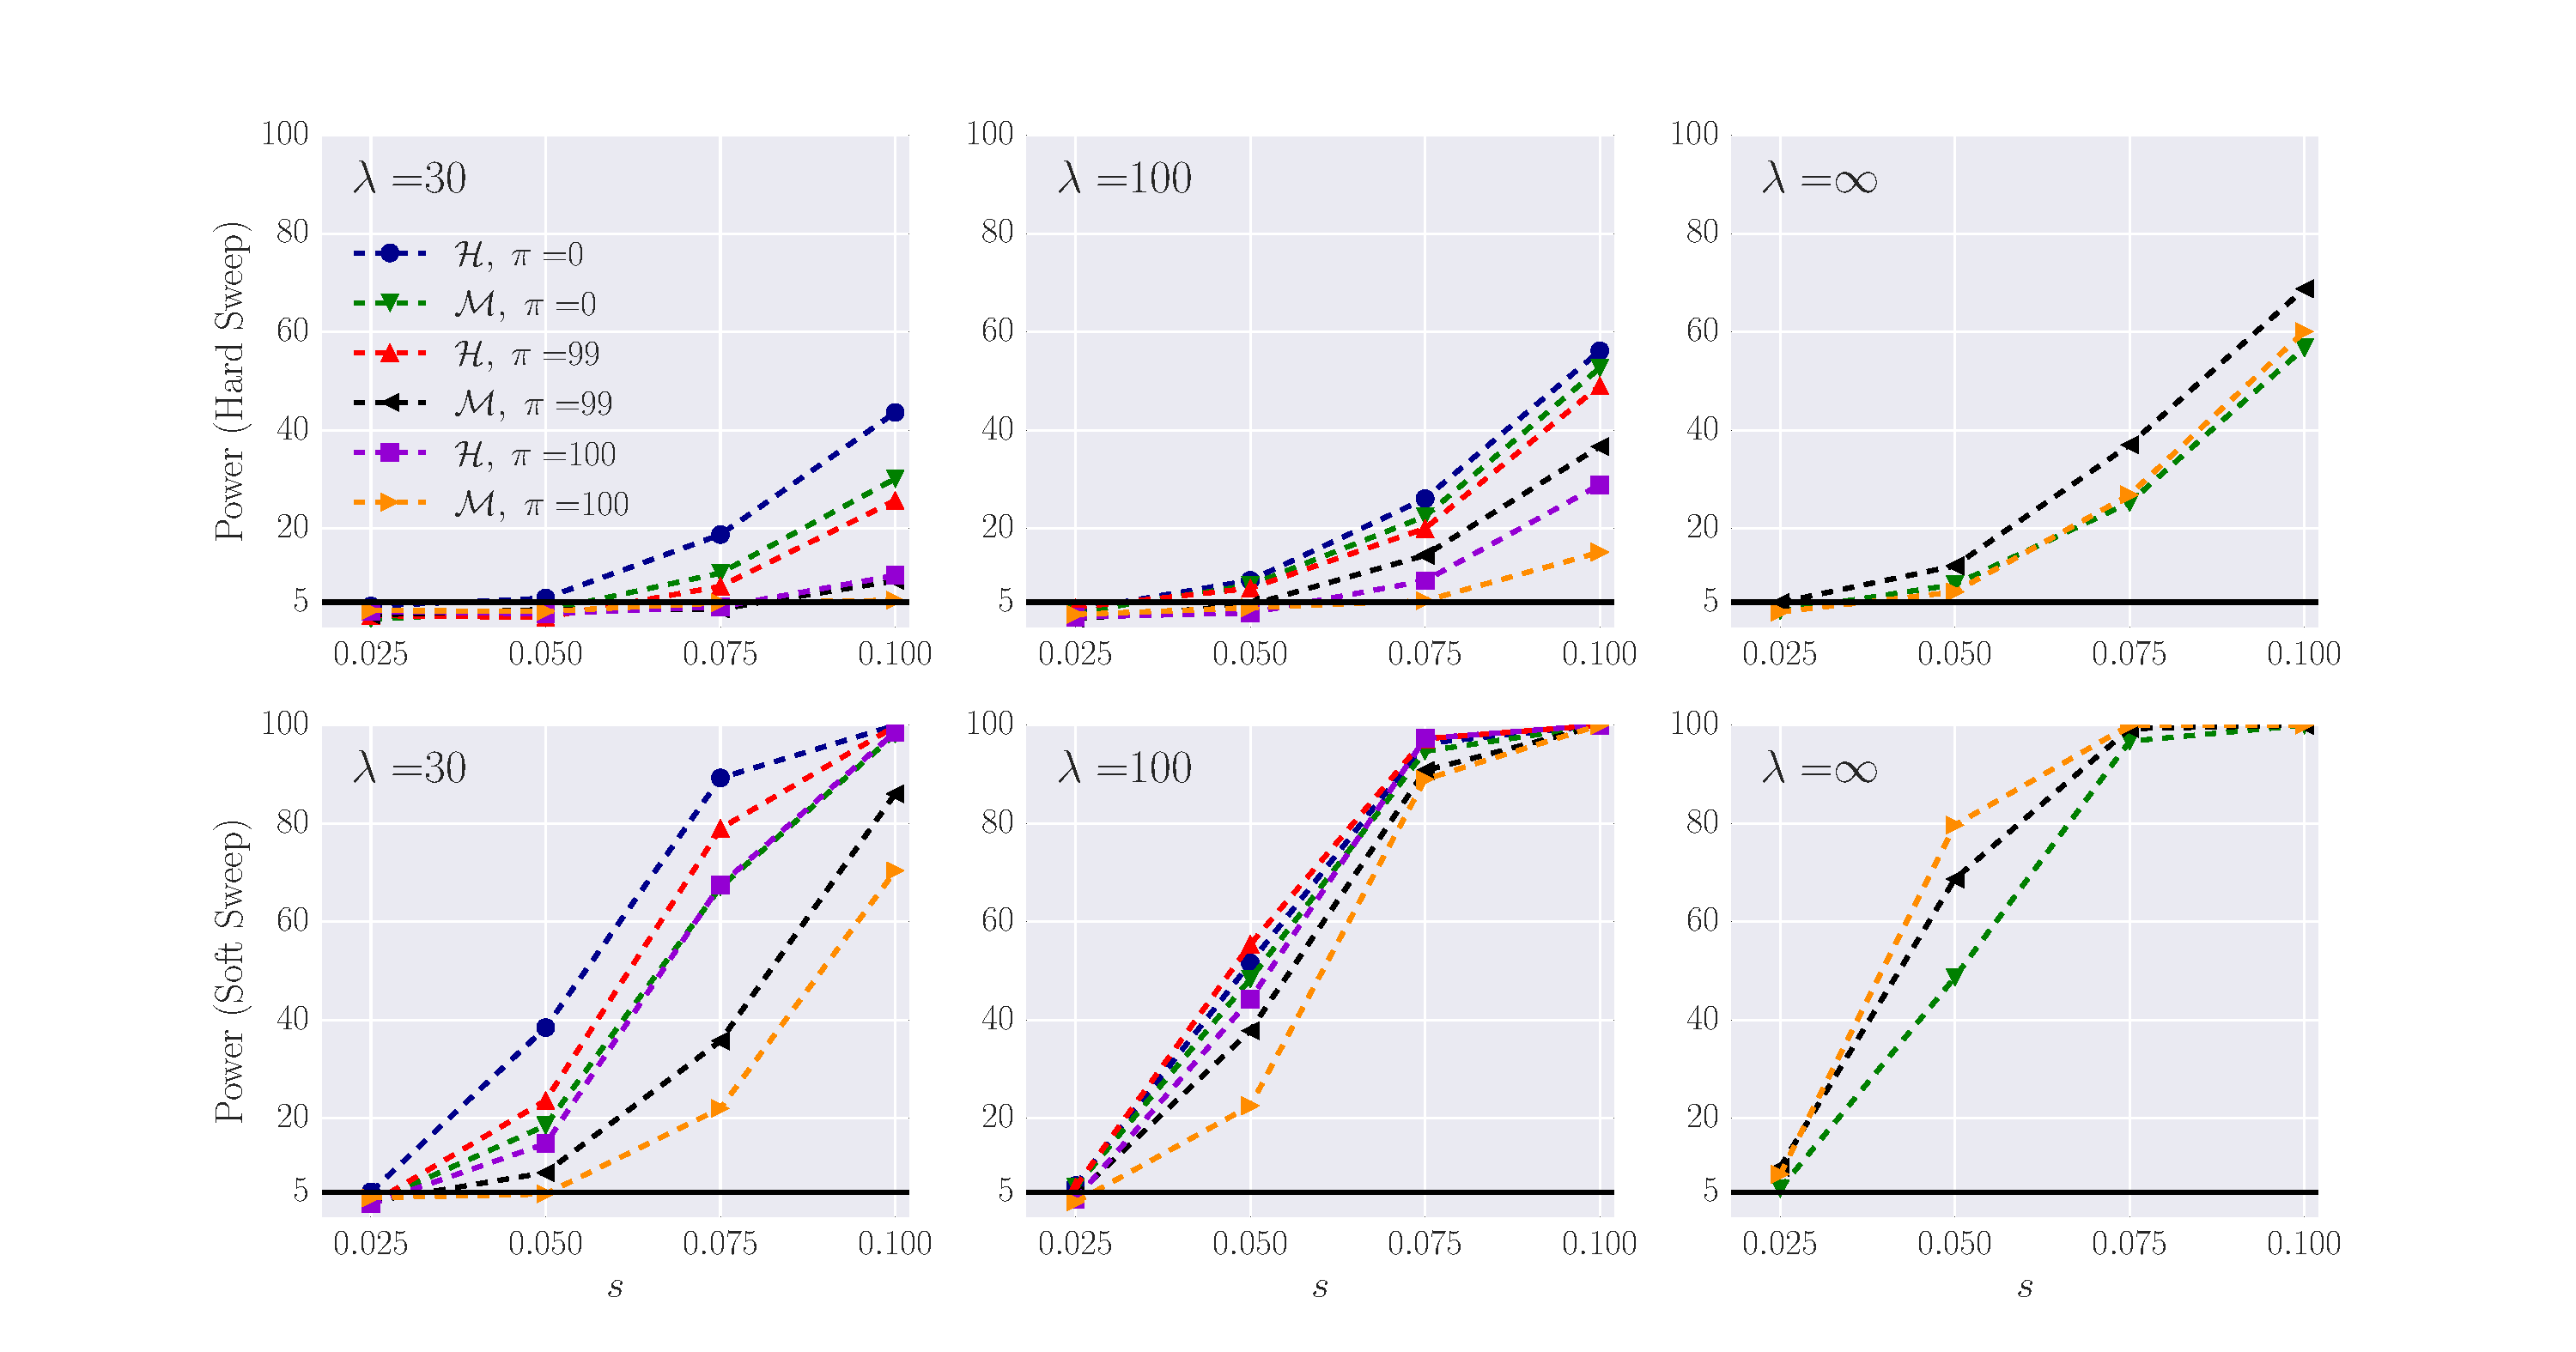
\includegraphics[width=\textwidth]{powerCLR.pdf}
	\caption{{\bf Comparison of power of Markov chain and HMM.}\\
          Detection power for Markov chain ($\Mc$) and HMM ($\Hc$) under 
          hard (A-C) and
          soft sweep (D-F) scenarios, for different coverage $\lambda$ and 
          selection strength $s$.  The
          $y$-axis measures power -- sensitivity with false positive
          rate FPR $\le 0.05$ -- for $2000$ simulations of $50$Kbp
          regions. The horizontal line reflects the power of a random
          classifier.
          In all simulations, 3 replicates are evolved and sampled at generations 
          $\Tc=\{0,10,20,30,40,50\}$.
           } \label{fig:powerCLR}
\end{figure}

\begin{figure}[H]
	\centering
	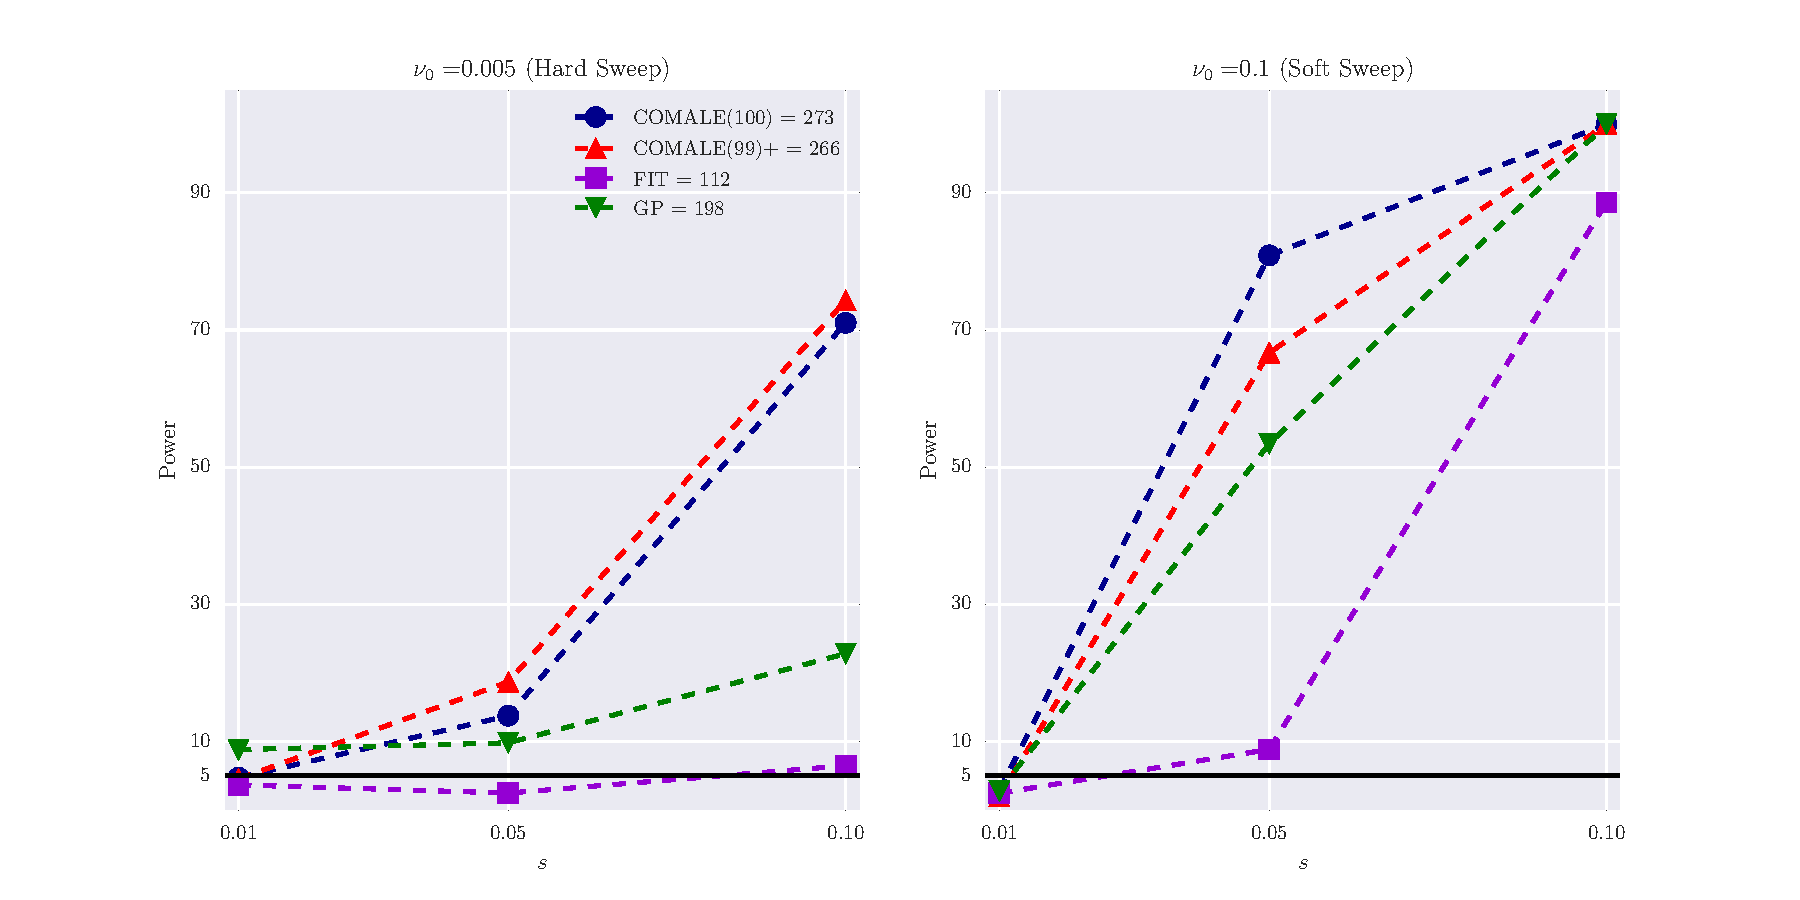
\includegraphics[width=\textwidth]{power.pdf}
	\caption{ {\bf Power calculations for detection of selection.}\\
          Detection power for \comale ($\Hc$), Frequency Increment
          Test (FIT), Gaussian Process (GP), and CMH under hard (A-C)
          and soft sweep (D-F) scenarios. $\lambda$, $s$ denote the
          mean coverage and selection coefficient, respectively. The
          $y$-axis measures power -- sensitivity with false positive
          rate FPR $\le 0.05$ -- for $2,000$ simulations of $50$Kbp
          regions. The horizontal line reflects the power of a random
          classifier.
          In all simulations, 3 replicates are evolved and sampled at generations 
          $\Tc=\{0,10,20,30,40,50\}$.}
           \label{fig:power}
\end{figure}

\begin{figure}[H]
	\centering
	\includegraphics[width=0.75\textwidth]{{runTime.pdf}}
	\caption{{\bf Running time.}\\ Box plots of running time per
          variant (CPU-secs.) of \comale ($\Mc$, $\Hc$), CMH, FIT, and
          GP with single, 3, 5, 7, and 10 loci over 1000 simulations
          conducted on a workstation with 4th Generation Intel Core i7
          processor. The average running time for each method is shown
          on the x-axis.
          In all simulations, 3 replicates are evolved and sampled at generations 
          $\Tc=\{0,10,20,30,40,50\}$.}
	\label{fig:runTime}
\end{figure}


\begin{figure}[H]
	\centering
	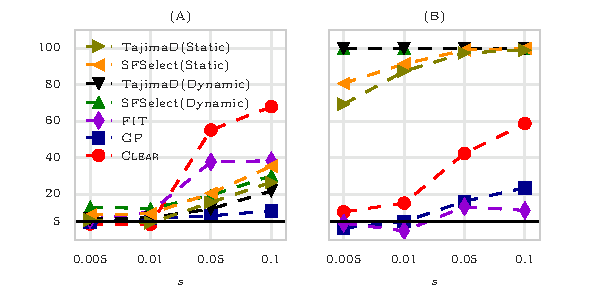
\includegraphics[width=0.7\textwidth]{naturalee.pdf}
	\caption{{\bf Power of SFS based statistics.}\\ Power of
          detecting selection for Frequency Increment Test (FIT),
          Gaussian Process (GP), \comale ($\Hc$) on hard sweep
          natural experimental evolution with $N_e=10^4$ and coverage
          $\lambda=\infty$. The measurements are conducted for a range
          of selection coefficients, $s$. Each point represents the
          mean of 200 simulations. For each simulation, sampling
          starts at a randomly chosen time, and subsequently 5
          replicate samples are acquired every $10$ generations.  (A)
          Start of sampling is chosen randomly throughout the sweep
          $\tau_1 \sim U\left[1,t_{\nu=1}(s,N_e)\right]$, where
          $t_{\nu=x}(s,N_e)$ denotes is the expected time to reach
          carrier frequency $x$ in a hard sweep and $U[a,b]$ is
          discrete uniform distribution. (B) The start of sampling is
          chosen near fixation of the favored allele, i.e. $\tau_1
          \sim
          U\left[t_{\nu=0.9}(s,N_e),t_{\nu=1}(s,N_e)\right]$.} 
          \label{fig:powerSFS}
\end{figure}

\begin{figure}[H]
	\centering
	\includegraphics[trim=.2in 0 .2in 0, 
	clip,width=\textwidth]{{rank100.0}.pdf}
	\caption{{\bf Ranking performance for 100$\times$ coverage.}\\
          Cumulative Distribution Function (CDF) of the distribution
          of the rank of the favored allele in 1000 simulations for
          \comale\ ($H$), Gaussian Process (GP), CMH, and Frequency
          Increment Test (FIT), for different values of selection
          coefficient $s$ and initial carrier frequency. Note that the
          individual variant \comale\ score ($H$) is used to rank
          variants.  The Area Under Curve (AUC) is computed as an overall
          quantitative measure to compare the performance of methods
          for each configuration. In all simulations, 3 replicates are evolved and 
          sampled at generations 
          $\Tc=\{0,10,20,30,40,50\}$.}
	\label{fig:rank}
\end{figure}



\begin{figure}[H]
	\centering
\includegraphics[width=0.7\textwidth]{{bias.100}.pdf}
\caption{{\bf Distribution of bias for 100$\times$ coverage.}\\ The
  distribution of bias ($s-\hat{s}$) in estimating selection
  coefficient over 1000 simulations using Gaussian Process (GP) and
  \comale\ ($H$) is shown for a range of choices for the selection
  coefficient $s$ and starting carrier frequency $\nu_0$, when
  coverage $\lambda=100$ (Panels A,B). GP and \comale\ have similar
  variance in estimates of $s$ for soft sweep, while \comale\ provides
  lower variance in hard sweep. Also see Table~\ref{tab:biasdist}. Panels C,D
  show the variance in the estimation of $h$. 
  In all simulations, 3 replicates are evolved and sampled at generations 
  $\Tc=\{0,10,20,30,40,50\}$.}
	\label{fig:bias100}
\end{figure}

\begin{figure}[H]
	\centering
	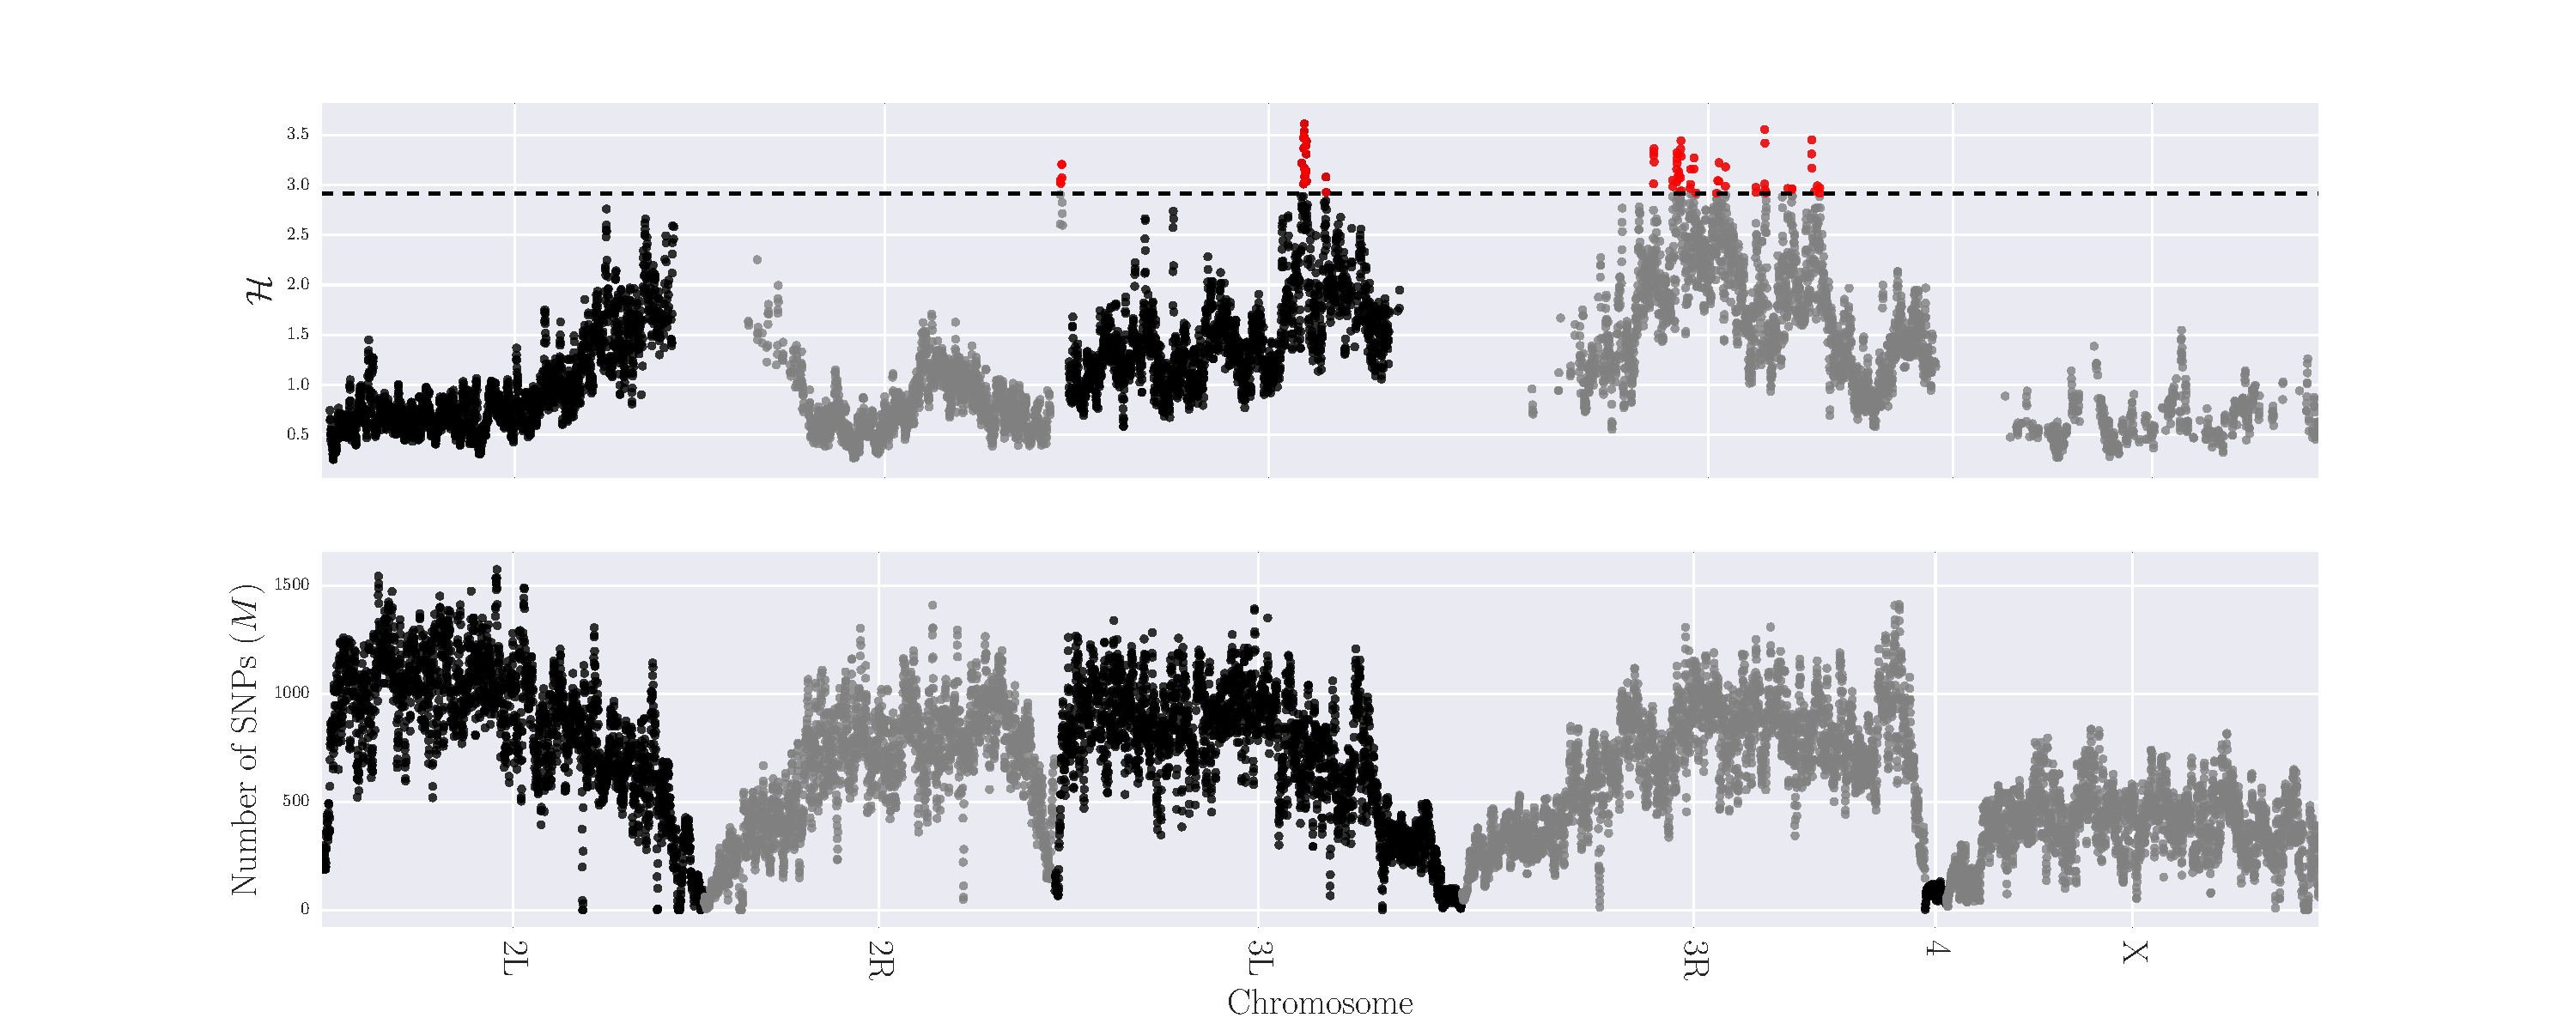
\includegraphics[width=\textwidth]{manhattan.pdf}
	\caption{{\bf \comale\ scan of the \datadm.}\\ Manhattan plot
          of the \comale\ ($\Hc^{+})$ statistic (A) and the number of
          SNPs (B) in 30Kbp sliding windows with steps of 10Kbp,
          excluding heterochromatic regions. Regions that exceed the local 
          FDR threshold of $\Hc^+$ are shown in
          red dots.}
	\label{fig:manhattancutoffed}
\end{figure}

\clearpage
\newpage